% ex: ts=2 sw=2 sts=2 et filetype=tex
% SPDX-License-Identifier: CC-BY-SA-4.0

\documentclass[12pt,addpoints]{exam}

\usepackage[utf8]{inputenc}
\usepackage[T1]{fontenc}
%\usepackage[spanish]{babel}
\usepackage[letterpaper]{geometry}

\pagestyle{headandfoot}
\headrule
\header{Física II}{Examen}{CBTIS 246}
\footer{}{Página \thepage\ de \numpages}{}

\pointpoints{punto}{puntos}
\renewcommand{\solutiontitle}{\textbf{Solución: }}


\newcommand{\makenonemptybox}[2]{%
  \par\nobreak\vspace{\ht\strutbox}\noindent
  \fbox{%
    \parbox[c][\dimexpr#1-2\fboxsep][t]{\dimexpr\linewidth-2\fboxsep}{
      \hrule width \hsize height 0pt
      #2
    }%
  }%
  \par\vspace{\ht\strutbox}
}
\makeatother

\printanswers

\begin{document}
%\begin{center}
%\fbox{\fbox{\parbox{5.5in}{\centering
%Lee con atención cada pregunta y responde en
%el espacio ubicado en la parte izquierda.
%}}}
%\end{center}
%
%\vspace{5mm}

Nombre:\enspace\hrulefill

\vspace{5mm}

Grupo:\enspace\hrulefill
\enspace{}Grado:\enspace\hrulefill
\enspace{}Fecha:\enspace\hrulefill

\begin{questions}

\input{p/p14t2}
% ex: ts=2 sw=2 sts=2 et filetype=tex
% SPDX-License-Identifier: CC-BY-SA-4.0

\question Las moléculas de los \fillin\ se pueden mover libremente debido a
  que la fuerza de atracción son más débil que en los sólidos, lo que permite
  que tengan mayor libertad de rotación y traslación, además de la vibración.

  \begin{oneparchoices}
    \CorrectChoice Líquidos
    \choice Plasma
    \choice Gaseosos
    \choice Sólidos
  \end{oneparchoices}
  \answerline[A]

% ex: ts=2 sw=2 sts=2 et filetype=tex
% SPDX-License-Identifier: CC-BY-SA-4.0

\question Es el conjunto donde la función esa definida, osea donde puede
tomar sus valores y realizar las operaciones qu se indican en  dicha
relación.


  \begin{oneparchoices}
    \choice Función
    \choice Dominio
    \choice Contradominio
    \choice Cuadratica
  \end{oneparchoices}
  %\answerline[A]

% ex: ts=2 sw=2 sts=2 et filetype=tex
% SPDX-License-Identifier: CC-BY-SA-4.0

\question Se realiza una fuerza \fillin \enspace, cuando un cuerpo empuja
          a otro.

  \begin{oneparchoices}
    \choice De empuje
    \CorrectChoice De contacto
    \choice De velocidad
    \choice De fricción
  \end{oneparchoices}
  \answerline[B]

% ex: ts=2 sw=2 sts=2 et filetype=tex
% SPDX-License-Identifier: CC-BY-SA-4.0

\question El prefijo \fillin \enspace del Sistema Internacional de Medidas
tiene un valor de $10^3$

  \begin{oneparchoices}
    \CorrectChoice kilo
    \choice micro
    \choice centi
    \choice deci
  \end{oneparchoices}
  \answerline[A]

% ex: ts=2 sw=2 sts=2 et filetype=tex
% SPDX-License-Identifier: CC-BY-SA-4.0

\question La \fillin \enspace ley de Newton establece que para cada acción
          hay una reacción.

  \begin{oneparchoices}
    \choice Cuarta
    \CorrectChoice Tercera
    \choice Segunda
    \choice Primera
  \end{oneparchoices}
  \answerline[B]

% ex: ts=2 sw=2 sts=2 et filetype=tex
% SPDX-License-Identifier: CC-BY-SA-4.0

\question Los \fillin\ se caracterizan porque las partículas que
los componen están muy cercanas entre sí, y en posiciones más o menos fijas

  \begin{oneparchoices}
    \choice Líquidos
    \CorrectChoice Sólidos
    \choice Gaseosos
    \choice Todos
  \end{oneparchoices}
  \answerline[B]

% ex: ts=2 sw=2 sts=2 et filetype=tex
% SPDX-License-Identifier: CC-BY-SA-4.0

\question Es la capacidad física para realizar un trabajo o un movimento.

  \begin{oneparchoices}
    \choice Rapidez
    \CorrectChoice Fuerza
    \choice Rozamiento
    \choice Aceleración
  \end{oneparchoices}
  \answerline[B]

% ex: ts=2 sw=2 sts=2 et filetype=tex
% SPDX-License-Identifier: CC-BY-SA-4.0

\question La formula de la ley de la dinamica es:

  \begin{oneparchoices}
    \CorrectChoice $F=m \cdot a$
    \choice $F=m \cdot v$
    \choice $F_{1 \rightarrow 2} = F_{2 \rightarrow 1}$
    \choice $\Sigma F = 0 \Leftrightarrow \frac{dv}{dt} = 0$
  \end{oneparchoices}
  \answerline[A]

% ex: ts=2 sw=2 sts=2 et filetype=tex
% SPDX-License-Identifier: CC-BY-SA-4.0

\question Usa la siguiente cuadricula para resolver los siguientes incisos:

  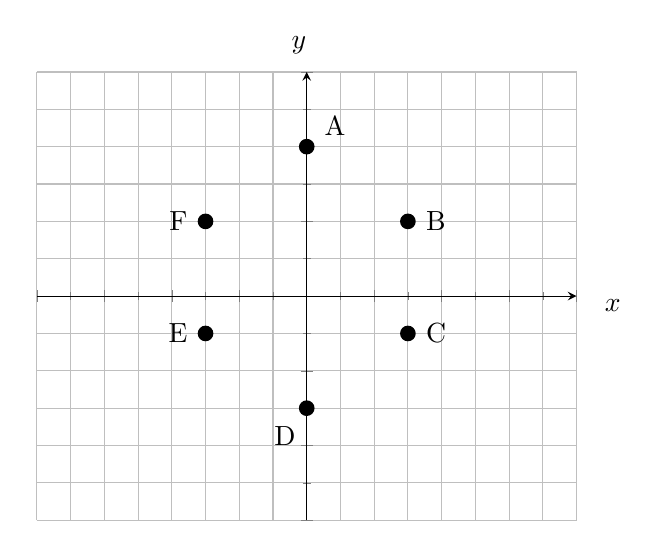
\begin{tikzpicture}
    \begin{axis}[grid=both,ymin=-6,ymax=6,xmax=8,xmin=-8,xticklabel=\empty,yticklabel=\empty,
               minor tick num=1,axis lines = middle,xlabel=$x$,ylabel=$y$,
               label style = {at={(ticklabel cs:1.1)}}]
      \node[label={10:{A}},circle,fill,inner sep=2pt] at (axis cs:0,4) {};
      \node[label={0:{B}},circle,fill,inner sep=2pt] at (axis cs:3,2) {};
      \node[label={0:{C}},circle,fill,inner sep=2pt] at (axis cs:3,-1) {};
      \node[label={260:{D}},circle,fill,inner sep=2pt] at (axis cs:0,-3) {};
      \node[label={180:{E}},circle,fill,inner sep=2pt] at (axis cs:-3,-1) {};
      \node[label={180:{F}},circle,fill,inner sep=2pt] at (axis cs:-3,2) {};
    \end{axis}
  \end{tikzpicture}

  \begin{parts}
    \part Encuantra las coordenadas de los vértices en el polígono. \\
    A(\fillin\ ,\fillin\ ) \enspace B(\fillin\ ,\fillin\ ) \\
    C(\fillin\ ,\fillin\ ) \enspace D(\fillin\ ,\fillin\ ) \\
    E(\fillin\ ,\fillin\ ) \enspace F(\fillin\ ,\fillin\ ) \\
    \part Determina el cuadrante en el que se ubica los puntos: \\
    El punto B esta en el cuadrante:\fillin \\
    El punto C esta en el cuadrante:\fillin \\
    El punto E esta en el cuadrante:\fillin \\
    El punto F esta en el cuadrante:\fillin \\
    \part Sacar la distancia entre los puntos: \\
    AB \fillin \enspace BC \fillin \enspace CD \fillin \\
    DE \fillin \enspace EF \fillin \enspace FA \fillin \\
    \part Calcula el perímetro de la figura resultante.
  \end{parts}

% ex: ts=2 sw=2 sts=2 et filetype=tex
% SPDX-License-Identifier: CC-BY-SA-4.0

\question Resuelve las siguientes ecuaciones y compruebalos sustituyendo el
          valor de $x$

  \begin{parts}
    \part $6x+4 = 3x+10$ \\
    \\
    \\
    \\
    \part $6x+3 = 2x+11$ \\
    \\
    \\
    \\
    \part $2x+5 = x-3$
  \end{parts}


\end{questions}

\end{document}
